\documentclass[12pt,aspectratio=169]{beamer}
\usepackage{ctex}  % 支持中文
\usepackage{tikz}  % 引入tikz包
\usepackage{minted}  % 用于源代码高亮显示

\title{TikZ 在 Beamer 中的应用示例}
\author{您的名字}
\date{\today}

\begin{document}

\frame{\titlepage}

\begin{frame}[fragile]
\frametitle{画点}

% 画点示例
\begin{minted}[frame=single,fontsize=\small]{latex}
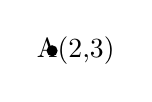
\begin{tikzpicture}
    % 画一个点
    \coordinate (A) at (2, 3);
    \fill (A) circle (2pt);
    % 标注点的名称和坐标
    \node at (2.3, 3) {A(2,3)};
\end{tikzpicture}
\end{minted}

% 显示画图结果
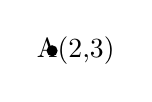
\begin{tikzpicture}
    \coordinate (A) at (2, 3);
    \fill (A) circle (2pt);
    \node at (2.3, 3) {A(2,3)};
\end{tikzpicture}
\end{frame}

\begin{frame}[fragile]
\frametitle{画三角形}

% 画三角形示例
\begin{minted}[frame=single,fontsize=\small]{latex}
\begin{tikzpicture}
    % 画三角形的三个点
    \coordinate (A) at (0, 0);
    \coordinate (B) at (4, 0);
    \coordinate (C) at (2, 3);
    
    % 画三角形
    \draw (A) -- (B) -- (C) -- cycle;
    
    % 标注点的名称和坐标
    \node at (A) [below left] {A(0,0)};
    \node at (B) [below right] {B(4,0)};
    \node at (C) [above] {C(2,3)};
\end{tikzpicture}
\end{minted}

% 显示画图结果
\begin{tikzpicture}
    \coordinate (A) at (0, 0);
    \coordinate (B) at (4, 0);
    \coordinate (C) at (2, 3);
    \draw (A) -- (B) -- (C) -- cycle;
    \node at (A) [below left] {A(0,0)};
    \node at (B) [below right] {B(4,0)};
    \node at (C) [above] {C(2,3)};
\end{tikzpicture}
\end{frame}

\begin{frame}[fragile]
\frametitle{画长方形}

% 画长方形示例
\begin{minted}[frame=single,fontsize=\small]{latex}
\begin{tikzpicture}
    % 定义四个顶点
    \coordinate (A) at (0, 0);
    \coordinate (B) at (4, 0);
    \coordinate (C) at (4, 2);
    \coordinate (D) at (0, 2);
    
    % 画长方形
    \draw (A) -- (B) -- (C) -- (D) -- cycle;
    
    % 标注点的名称和坐标
    \node at (A) [below left] {A(0,0)};
    \node at (B) [below right] {B(4,0)};
    \node at (C) [above right] {C(4,2)};
    \node at (D) [above left] {D(0,2)};
\end{tikzpicture}
\end{minted}

% 显示画图结果
\begin{tikzpicture}
    \coordinate (A) at (0, 0);
    \coordinate (B) at (4, 0);
    \coordinate (C) at (4, 2);
    \coordinate (D) at (0, 2);
    \draw (A) -- (B) -- (C) -- (D) -- cycle;
    \node at (A) [below left] {A(0,0)};
    \node at (B) [below right] {B(4,0)};
    \node at (C) [above right] {C(4,2)};
    \node at (D) [above left] {D(0,2)};
\end{tikzpicture}
\end{frame}

\begin{frame}[fragile]
\frametitle{画圆和椭圆}

% 画圆和椭圆示例
\begin{minted}[frame=single,fontsize=\small]{latex}
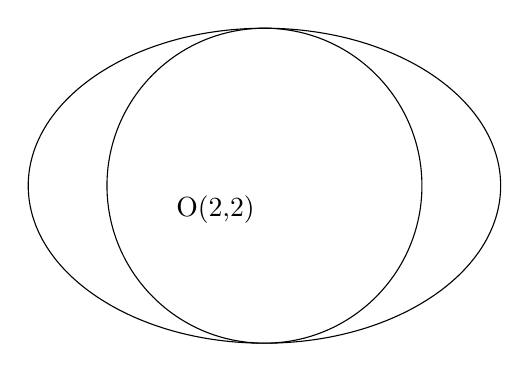
\begin{tikzpicture}
    % 画圆,圆心为O(2,2),半径为2
    \draw (2, 2) circle (2cm);
    \node at (2, 2) [below left] {O(2,2)};
    
    % 画椭圆,中心在(2,2),长轴为3,短轴为2
    \draw (2, 2) ellipse (3cm and 2cm);
\end{tikzpicture}
\end{minted}

% 显示画图结果
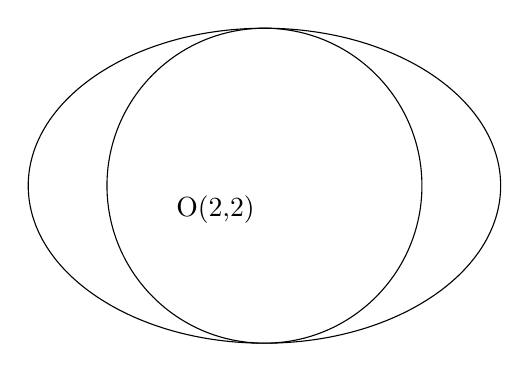
\begin{tikzpicture}
    \draw (2, 2) circle (2cm);
    \node at (2, 2) [below left] {O(2,2)};
    \draw (2, 2) ellipse (3cm and 2cm);
\end{tikzpicture}
\end{frame}

\begin{frame}[fragile]
\frametitle{画圆弧}

% 画圆弧示例
\begin{minted}[frame=single,fontsize=\small]{latex}
\begin{tikzpicture}
    % 画圆弧,圆心为O(0,0),半径为3,角度从0到90度
    \draw (0,0) arc[start angle=0, end angle=90, radius=3cm];
    \node at (0, 0) [below left] {O(0,0)};
\end{tikzpicture}
\end{minted}

% 显示画图结果
\begin{tikzpicture}
    \draw (0,0) arc[start angle=0, end angle=90, radius=3cm];
    \node at (0, 0) [below left] {O(0,0)};
\end{tikzpicture}
\end{frame}

\end{document}
